\documentclass{article}
\usepackage{tikz}
\usepackage{amsmath,amssymb}
\pagestyle{empty}
\pdfpagewidth=21cm
\pdfpageheight=20cm
\oddsidemargin=-1in
\topmargin=-1in
\headheight=0pt
\headsep=0pt
\textwidth=21cm
\textheight=20cm
\hoffset=0.5cm
\voffset=0.5cm
\usetikzlibrary{
  arrows.meta,
  positioning,
  shapes.geometric,
  fit,
  calc,
  decorations.pathreplacing,
  backgrounds,
  matrix
}

\definecolor{rank0}{RGB}{66,133,244}
\definecolor{rank1}{RGB}{234,67,53}
\definecolor{rank2}{RGB}{52,168,83}
\definecolor{avcolor}{RGB}{144,202,249}
\definecolor{thcolor}{RGB}{255,183,77}
\definecolor{partcolor}{RGB}{200,230,201}
\definecolor{mutexcolor}{RGB}{206,147,216}
\definecolor{rdmacolor}{RGB}{255,112,67}
\definecolor{arrowblue}{RGB}{30,90,180}
\definecolor{darkbg}{RGB}{248,248,255}
\definecolor{selfbg}{RGB}{230,240,255}
\definecolor{remotebg}{RGB}{255,245,230}

\newcommand{\circled}[1]{%
  \tikz[baseline=(char.base)]{
    \node[shape=circle, draw, inner sep=1pt, minimum size=10pt,
          font=\sffamily\tiny\bfseries, thick] (char) {#1};
  }%
}

% ---------------------------------------------------------------
% Macro: draw one mini RankHandler cell (centered content)
%   #1 = x,  #2 = y,  #3 = bg color,  #4 = label,
%   #5 = show lock (1/0),  #6 = th active count,  #7 = av active count
% ---------------------------------------------------------------
\newcommand{\drawHandler}[7]{%
  \begin{scope}[shift={(#1,#2)}]
    \fill[#3, rounded corners=3pt] (-2.3,-1.1) rectangle (2.3,1.25);
    \draw[gray!60, rounded corners=3pt] (-2.3,-1.1) rectangle (2.3,1.25);
    % -- particles[] --
    \node[font=\sffamily\tiny\bfseries, anchor=east] at (-1.55, 0.85) {P};
    \foreach \i in {0,...,7} {
      \pgfmathsetmacro{\xc}{-1.35 + \i*0.38}
      \fill[partcolor, draw=partcolor!60!black, thin]
        (\xc-0.16, 0.69) rectangle (\xc+0.16, 1.01);
    }
    % -- th[] --
    \node[font=\sffamily\tiny\bfseries, anchor=east, thcolor!80!black] at (-1.55, 0.35) {th};
    \foreach \i in {0,...,7} {
      \pgfmathsetmacro{\xc}{-1.35 + \i*0.38}
      \ifnum \i<#6
        \fill[thcolor, draw=thcolor!60!black, thin]
          (\xc-0.16, 0.19) rectangle (\xc+0.16, 0.51);
      \else
        \fill[thcolor!15, draw=thcolor!80!black, thin]
          (\xc-0.16, 0.19) rectangle (\xc+0.16, 0.51);
      \fi
    }
    % th length right after array
    \node[font=\sffamily\tiny\bfseries, thcolor!60!black, anchor=west] at (1.55, 0.35) {#6};
    % -- av[] --
    \node[font=\sffamily\tiny\bfseries, anchor=east, avcolor!80!black] at (-1.55, -0.2) {av};
    \foreach \i in {0,...,7} {
      \pgfmathsetmacro{\xc}{-1.35 + \i*0.38}
      \ifnum \i<#7
        \fill[avcolor, draw=avcolor!60!black, thin]
          (\xc-0.16, -0.36) rectangle (\xc+0.16, -0.04);
      \else
        \fill[avcolor!15, draw=avcolor!80!black, thin]
          (\xc-0.16, -0.36) rectangle (\xc+0.16, -0.04);
      \fi
    }
    % av length right after array
    \node[font=\sffamily\tiny\bfseries, avcolor!60!black, anchor=west] at (1.55, -0.2) {#7};
    % -- lock --
    \ifnum#5=1
      \node[draw=mutexcolor!80!black, fill=mutexcolor!20, rounded corners=1pt,
            font=\sffamily\tiny, inner sep=2pt, minimum width=1.0cm]
        at (0, -0.8) {\texttt{mutex}};
    \else
      \node[font=\sffamily\tiny, gray!50, inner sep=2pt] at (0, -0.8) {(no lock)};
    \fi
  \end{scope}
}

\begin{document}

% =====================================================================
% PAGE 1: The Matrix View
% =====================================================================
\pdfpageheight=16cm
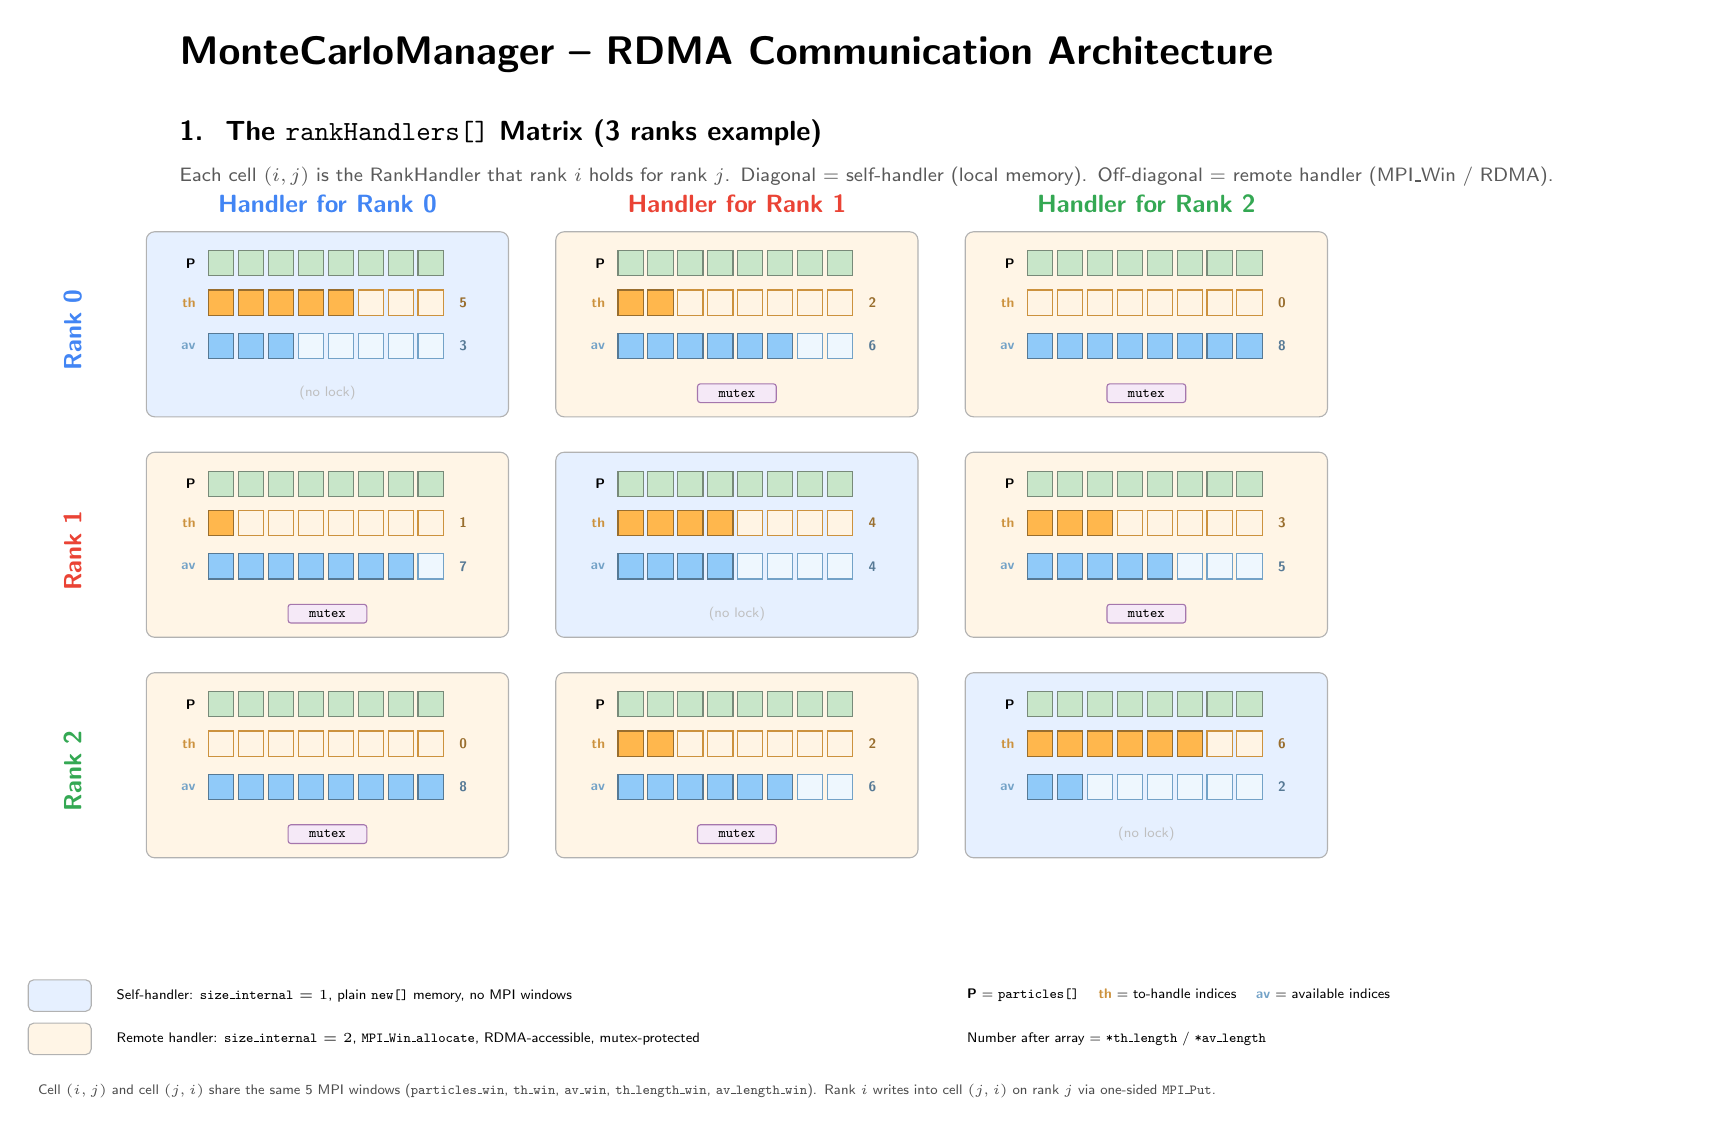
\begin{tikzpicture}[>=Stealth, font=\sffamily\small]

  \node[font=\sffamily\Large\bfseries, anchor=west] at (-1, 0)
    {MonteCarloManager -- RDMA Communication Architecture};

  \node[font=\sffamily\normalsize\bfseries, anchor=west] at (-1, -1.0)
    {1.\; The \texttt{rankHandlers[]} Matrix (3 ranks example)};
  \node[font=\sffamily\scriptsize, anchor=west, text=gray!70!black, text width=19cm]
    at (-1, -1.55)
    {Each cell $(i,j)$ is the RankHandler that rank $i$ holds for rank $j$.
     Diagonal = self-handler (local memory).
     Off-diagonal = remote handler (MPI\_Win / RDMA).};

  \begin{scope}[shift={(0, -5.5)}]
    % Column headers
    \node[font=\sffamily\small\bfseries, rank0] at (1.0, 3.6) {Handler for Rank 0};
    \node[font=\sffamily\small\bfseries, rank1] at (6.2, 3.6) {Handler for Rank 1};
    \node[font=\sffamily\small\bfseries, rank2] at (11.4, 3.6) {Handler for Rank 2};

    % Row headers
    \node[font=\sffamily\small\bfseries, rank0, rotate=90, anchor=south]
      at (-2.0, 2.0) {Rank 0};
    \node[font=\sffamily\small\bfseries, rank1, rotate=90, anchor=south]
      at (-2.0, -0.8) {Rank 1};
    \node[font=\sffamily\small\bfseries, rank2, rotate=90, anchor=south]
      at (-2.0, -3.6) {Rank 2};

    % Row 0: Rank 0's handlers           bg            label                   lock th av
    \drawHandler{1.0}{2.0}  {selfbg}  {self (\texttt{new[]})}{0}{5}{3}
    \drawHandler{6.2}{2.0}  {remotebg}{MPI\_Win (RDMA)}      {1}{2}{6}
    \drawHandler{11.4}{2.0} {remotebg}{MPI\_Win (RDMA)}      {1}{0}{8}
    % Row 1: Rank 1's handlers
    \drawHandler{1.0}{-0.8} {remotebg}{MPI\_Win (RDMA)}      {1}{1}{7}
    \drawHandler{6.2}{-0.8} {selfbg}  {self (\texttt{new[]})}{0}{4}{4}
    \drawHandler{11.4}{-0.8}{remotebg}{MPI\_Win (RDMA)}      {1}{3}{5}
    % Row 2: Rank 2's handlers
    \drawHandler{1.0}{-3.6} {remotebg}{MPI\_Win (RDMA)}      {1}{0}{8}
    \drawHandler{6.2}{-3.6} {remotebg}{MPI\_Win (RDMA)}      {1}{2}{6}
    \drawHandler{11.4}{-3.6}{selfbg}  {self (\texttt{new[]})}{0}{6}{2}
  \end{scope}

  % Legend
  \begin{scope}[shift={(0, -12.2)}]
    \fill[selfbg, draw=gray!60, rounded corners=2pt] (-2.8, 0.05) rectangle (-2.0, 0.45);
    \node[font=\sffamily\tiny, anchor=west] at (-1.8, 0.25)
      {Self-handler: \texttt{size\_internal}${}=1$, plain \texttt{new[]} memory, no MPI windows};

    \fill[remotebg, draw=gray!60, rounded corners=2pt] (-2.8, -0.5) rectangle (-2.0, -0.1);
    \node[font=\sffamily\tiny, anchor=west] at (-1.8, -0.3)
      {Remote handler: \texttt{size\_internal}${}=2$, \texttt{MPI\_Win\_allocate}, RDMA-accessible, mutex-protected};

    \node[font=\sffamily\tiny, anchor=west] at (9.0, 0.25) {%
      \textbf{P} = \texttt{particles[]} \quad
      \textcolor{thcolor!80!black}{\textbf{th}} = to-handle indices \quad
      \textcolor{avcolor!80!black}{\textbf{av}} = available indices};
    \node[font=\sffamily\tiny, anchor=west] at (9.0, -0.3) {%
      Number after array = \texttt{*th\_length} / \texttt{*av\_length}};

    \node[font=\sffamily\tiny, anchor=north west, text=gray!60!black, text width=19cm]
      at (-2.8, -0.75) {%
      Cell $(i,j)$ and cell $(j,i)$ share the same 5 MPI windows
      (\texttt{particles\_win}, \texttt{th\_win}, \texttt{av\_win},
      \texttt{th\_length\_win}, \texttt{av\_length\_win}).
      Rank $i$ writes into cell $(j,i)$ on rank $j$ via one-sided \texttt{MPI\_Put}.};
  \end{scope}

\end{tikzpicture}

% =====================================================================
% PAGE 2: Detailed Buffer Layout
% =====================================================================
\newpage
\pdfpageheight=13cm
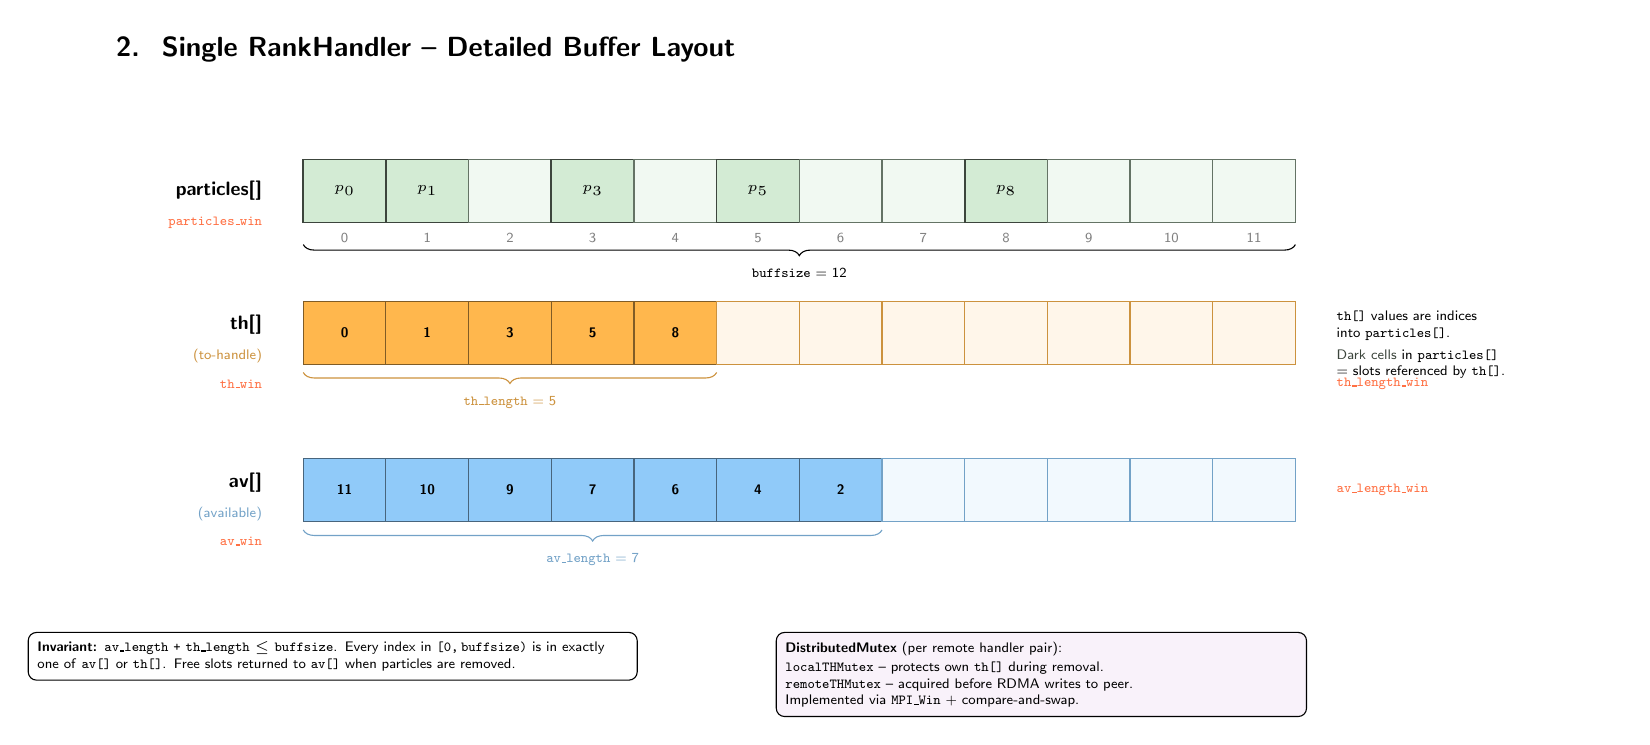
\begin{tikzpicture}[>=Stealth, font=\sffamily\small]

  \node[font=\sffamily\normalsize\bfseries, anchor=west] at (-1, 0)
    {2.\; Single RankHandler -- Detailed Buffer Layout};

  \begin{scope}[shift={(1.5, -1.5)}]
    \def\cw{1.05}
    \def\xstart{0}

    % ---- particles[] ----
    \node[font=\sffamily\scriptsize\bfseries, anchor=east] at (-0.4, -0.3) {particles[]};
    \node[font=\sffamily\tiny, anchor=east, rdmacolor] at (-0.4, -0.7)
      {\texttt{particles\_win}};

    % occupied indices (referenced by th[]): darker fill + thick border
    \foreach \i in {0,...,11} {
      \pgfmathsetmacro{\xl}{\xstart + \i*\cw}
      \pgfmathsetmacro{\xr}{\xl + \cw}
      % check if this index is in the th set {0,1,3,5,8}
      \pgfmathsetmacro{\isactive}{(\i==0)||(\i==1)||(\i==3)||(\i==5)||(\i==8)?1:0}
      \ifnum \isactive>0
        \fill[partcolor!80, draw=partcolor!30!black, semithick]
          (\xl, -0.7) rectangle (\xr, 0.1);
      \else
        \fill[partcolor!25, draw=partcolor!50!black, thin]
          (\xl, -0.7) rectangle (\xr, 0.1);
      \fi
    }
    \foreach \i/\lab in {0/$p_0$, 1/$p_1$, 2/\phantom{-}, 3/$p_3$, 4/\phantom{-}, 5/$p_5$,
                          6/\phantom{-}, 7/\phantom{-}, 8/$p_8$, 9/\phantom{-}, 10/\phantom{-}, 11/\phantom{-}} {
      \pgfmathsetmacro{\xc}{\xstart + \i*\cw + 0.5*\cw}
      \node[font=\sffamily\tiny] at (\xc, -0.3) {\lab};
    }
    % index labels below
    \foreach \i in {0,...,11} {
      \pgfmathsetmacro{\xc}{\xstart + \i*\cw + 0.5*\cw}
      \node[font=\sffamily\tiny, gray] at (\xc, -0.9) {\i};
    }

    % buffsize brace below
    \pgfmathsetmacro{\xleft}{\xstart}
    \pgfmathsetmacro{\xright}{\xstart + 12*\cw}
    \draw[decorate, decoration={brace, amplitude=4pt, mirror, raise=8pt}]
      (\xleft, -0.7) -- (\xright, -0.7)
      node[midway, below=13pt, font=\sffamily\tiny] {\texttt{buffsize} = 12};

    % ---- th[] (to-handle) ----
    \def\thy{-2.4}
    \node[font=\sffamily\scriptsize\bfseries, anchor=east] at (-0.4, \thy+0.4) {th[]};
    \node[font=\sffamily\tiny, anchor=east, thcolor!80!black] at (-0.4, \thy)
      {(to-handle)};
    \node[font=\sffamily\tiny, anchor=east, rdmacolor] at (-0.4, \thy-0.35)
      {\texttt{th\_win}};

    \foreach \i in {0,...,11} {
      \pgfmathsetmacro{\xl}{\xstart + \i*\cw}
      \pgfmathsetmacro{\xr}{\xl + \cw}
      \ifnum \i<5
        \fill[thcolor, draw=thcolor!50!black, thin]
          (\xl, \thy-0.1) rectangle (\xr, \thy+0.7);
      \else
        \fill[thcolor!12, draw=thcolor!80!black, thin]
          (\xl, \thy-0.1) rectangle (\xr, \thy+0.7);
      \fi
    }
    \foreach \i/\val in {0/0, 1/1, 2/3, 3/5, 4/8} {
      \pgfmathsetmacro{\xc}{\xstart + \i*\cw + 0.5*\cw}
      \node[font=\sffamily\tiny\bfseries] at (\xc, \thy+0.3) {\val};
    }

    % th_length: brace below the active portion
    \pgfmathsetmacro{\thright}{\xstart + 5*\cw}
    \draw[decorate, decoration={brace, amplitude=4pt, mirror, raise=3pt}, thcolor!80!black]
      (\xleft, \thy-0.1) -- (\thright, \thy-0.1)
      node[midway, below=8pt, font=\sffamily\tiny, thcolor!80!black]
      {\texttt{th\_length} = 5};

    % Annotation: th values are indices into particles (instead of arrows)
    \pgfmathsetmacro{\annotx}{\xright + 0.4}
    \node[font=\sffamily\tiny, anchor=north west, text width=3.5cm, align=left]
      at (\annotx, \thy+0.7) {%
        \texttt{th[]} values are indices\\
        into \texttt{particles[]}.\\[2pt]
        \textcolor{partcolor!30!black}{Dark cells} in \texttt{particles[]}\\
        = slots referenced by \texttt{th[]}.};

    % ---- av[] (available) ----
    \def\avy{-4.4}
    \node[font=\sffamily\scriptsize\bfseries, anchor=east] at (-0.4, \avy+0.4) {av[]};
    \node[font=\sffamily\tiny, anchor=east, avcolor!80!black] at (-0.4, \avy)
      {(available)};
    \node[font=\sffamily\tiny, anchor=east, rdmacolor] at (-0.4, \avy-0.35)
      {\texttt{av\_win}};

    \foreach \i in {0,...,11} {
      \pgfmathsetmacro{\xl}{\xstart + \i*\cw}
      \pgfmathsetmacro{\xr}{\xl + \cw}
      \ifnum \i<7
        \fill[avcolor, draw=avcolor!50!black, thin]
          (\xl, \avy-0.1) rectangle (\xr, \avy+0.7);
      \else
        \fill[avcolor!12, draw=avcolor!80!black, thin]
          (\xl, \avy-0.1) rectangle (\xr, \avy+0.7);
      \fi
    }
    \foreach \i/\val in {0/11, 1/10, 2/9, 3/7, 4/6, 5/4, 6/2} {
      \pgfmathsetmacro{\xc}{\xstart + \i*\cw + 0.5*\cw}
      \node[font=\sffamily\tiny\bfseries] at (\xc, \avy+0.3) {\val};
    }

    % av_length: brace below the active portion
    \pgfmathsetmacro{\avright}{\xstart + 7*\cw}
    \draw[decorate, decoration={brace, amplitude=4pt, mirror, raise=3pt}, avcolor!80!black]
      (\xleft, \avy-0.1) -- (\avright, \avy-0.1)
      node[midway, below=8pt, font=\sffamily\tiny, avcolor!80!black]
      {\texttt{av\_length} = 7};

    % MPI Win labels on the right
    \node[font=\sffamily\tiny, anchor=west, rdmacolor] at (\annotx, \thy-0.35)
      {\texttt{th\_length\_win}};
    \node[font=\sffamily\tiny, anchor=west, rdmacolor] at (\annotx, \avy+0.3)
      {\texttt{av\_length\_win}};

    % ---- Notes at bottom ----
    \node[draw, rounded corners=3pt, fill=white, font=\sffamily\tiny,
          text width=7.5cm, align=left, anchor=north west] at (-3.5, -5.9) {
      \textbf{Invariant:} \texttt{av\_length + th\_length $\leq$ buffsize}.
      Every index in \texttt{[0,\,buffsize)} is in exactly one of
      \texttt{av[]} or \texttt{th[]}. Free slots returned to \texttt{av[]}
      when particles are removed.
    };
    \node[draw, rounded corners=3pt, fill=mutexcolor!12, font=\sffamily\tiny,
          text width=6.5cm, align=left, anchor=north west] at (6.0, -5.9) {
      \textbf{DistributedMutex} (per remote handler pair):\\[1pt]
      \texttt{localTHMutex} -- protects own \texttt{th[]} during removal.\\
      \texttt{remoteTHMutex} -- acquired before RDMA writes to peer.\\
      Implemented via \texttt{MPI\_Win} + compare-and-swap.
    };
  \end{scope}

\end{tikzpicture}

% =====================================================================
% PAGE 3: RDMA Transfer Protocol
% =====================================================================
\newpage
\pdfpageheight=13cm
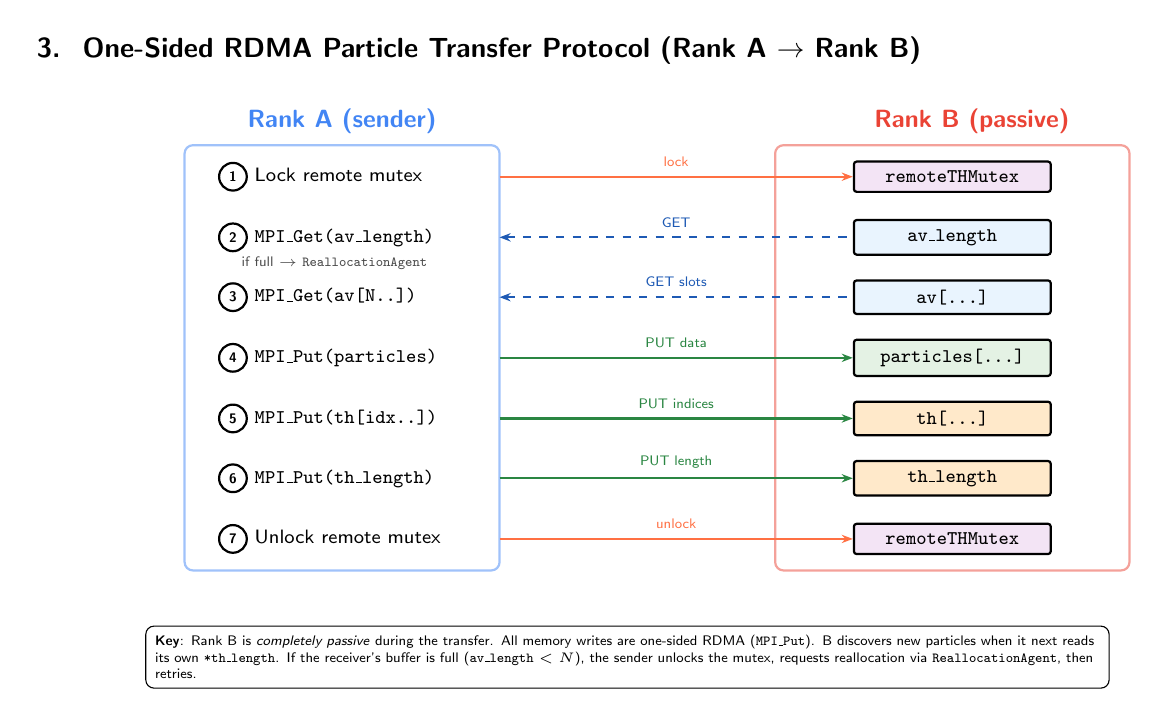
\begin{tikzpicture}[>=Stealth, font=\sffamily\small]

  \node[font=\sffamily\normalsize\bfseries, anchor=west] at (-1, 0)
    {3.\; One-Sided RDMA Particle Transfer Protocol (Rank A $\to$ Rank B)};

  \begin{scope}[shift={(0, -6.7)}]
    % Rank A box (centered left)
    \node[font=\sffamily\small\bfseries, rank0] at (3.0, 5.8) {Rank A (sender)};
    \draw[rank0!50, thick, rounded corners=3pt] (1.0, 0.1) rectangle (5.0, 5.5);

    % Rank B box (centered right, closer)
    \node[font=\sffamily\small\bfseries, rank1] at (11.0, 5.8) {Rank B (passive)};
    \draw[rank1!50, thick, rounded corners=3pt] (8.5, 0.1) rectangle (13.0, 5.5);

    \tikzset{
      wbox/.style={draw, thick, fill=#1, minimum width=2.5cm,
                   minimum height=0.32cm, font=\sffamily\scriptsize,
                   rounded corners=1pt}
    }

    % 7 steps equally spaced: y from 5.1 down to 0.5, step = 0.767
    \def\ystepA{5.10}
    \def\ystepB{4.33}
    \def\ystepC{3.57}
    \def\ystepD{2.80}
    \def\ystepE{2.03}
    \def\ystepF{1.27}
    \def\ystepG{0.50}

    % Rank B components at each step
    \node[wbox=mutexcolor!25] (bmutex)  at (10.75, \ystepA) {\texttt{remoteTHMutex}};
    \node[wbox=avcolor!20]    (bavl)    at (10.75, \ystepB) {\texttt{av\_length}};
    \node[wbox=avcolor!20]    (bav)     at (10.75, \ystepC) {\texttt{av[...]}};
    \node[wbox=partcolor!50]  (bpart)   at (10.75, \ystepD) {\texttt{particles[...]}};
    \node[wbox=thcolor!30]    (bth)     at (10.75, \ystepE) {\texttt{th[...]}};
    \node[wbox=thcolor!30]    (bthl)    at (10.75, \ystepF) {\texttt{th\_length}};
    \node[wbox=mutexcolor!25] (bmutex2) at (10.75, \ystepG) {\texttt{remoteTHMutex}};

    % Steps: left-aligned inside Rank A box
    \def\sx{1.3}
    \node[font=\sffamily\scriptsize, anchor=west] at (\sx, \ystepA)
      {\circled{1} Lock remote mutex};
    \node[font=\sffamily\scriptsize, anchor=west] at (\sx, \ystepB)
      {\circled{2} \texttt{MPI\_Get(av\_length)}};
    \node[font=\sffamily\tiny, anchor=west, gray!60!black] at (1.6, 4.0)
      {if full $\to$ \texttt{ReallocationAgent}};
    \node[font=\sffamily\scriptsize, anchor=west] at (\sx, \ystepC)
      {\circled{3} \texttt{MPI\_Get(av[N..])}};
    \node[font=\sffamily\scriptsize, anchor=west] at (\sx, \ystepD)
      {\circled{4} \texttt{MPI\_Put(particles)}};
    \node[font=\sffamily\scriptsize, anchor=west] at (\sx, \ystepE)
      {\circled{5} \texttt{MPI\_Put(th[idx..])}};
    \node[font=\sffamily\scriptsize, anchor=west] at (\sx, \ystepF)
      {\circled{6} \texttt{MPI\_Put(th\_length)}};
    \node[font=\sffamily\scriptsize, anchor=west] at (\sx, \ystepG)
      {\circled{7} Unlock remote mutex};

    % Arrows between boxes
    \def\ax{5.0}
    % lock/unlock: A → B
    \draw[-{Stealth[length=4pt]}, rdmacolor, thick]
      (\ax, \ystepA) -- (bmutex.west)
      node[midway, above, font=\sffamily\tiny, sloped] {lock};
    % GET: arrow from B to A (data flows back)
    \draw[{Stealth[length=4pt]}-, arrowblue, thick, dashed]
      (\ax, \ystepB) -- (bavl.west)
      node[midway, above, font=\sffamily\tiny, sloped] {GET};
    \draw[{Stealth[length=4pt]}-, arrowblue, thick, dashed]
      (\ax, \ystepC) -- (bav.west)
      node[midway, above, font=\sffamily\tiny, sloped] {GET slots};
    % PUT: A → B
    \draw[-{Stealth[length=4pt]}, rank2!80!black, thick]
      (\ax, \ystepD) -- (bpart.west)
      node[midway, above, font=\sffamily\tiny, sloped] {PUT data};
    \draw[-{Stealth[length=4pt]}, rank2!80!black, thick]
      (\ax, \ystepE) -- (bth.west)
      node[midway, above, font=\sffamily\tiny, sloped] {PUT indices};
    \draw[-{Stealth[length=4pt]}, rank2!80!black, thick]
      (\ax, \ystepF) -- (bthl.west)
      node[midway, above, font=\sffamily\tiny, sloped] {PUT length};
    \draw[-{Stealth[length=4pt]}, rdmacolor, thick]
      (\ax, \ystepG) -- (bmutex2.west)
      node[midway, above, font=\sffamily\tiny, sloped] {unlock};
  \end{scope}

  % Key note below the figure
  \node[draw, rounded corners=3pt, fill=white, font=\sffamily\tiny,
        text width=12cm, align=left, anchor=north west] at (0.5, -7.3) {
    \textbf{Key}: Rank B is \emph{completely passive} during the transfer.
    All memory writes are one-sided RDMA (\texttt{MPI\_Put}).
    B discovers new particles when it next reads its own \texttt{*th\_length}.
    If the receiver's buffer is full (\texttt{av\_length} $<$ $N$), the sender
    unlocks the mutex, requests reallocation via \texttt{ReallocationAgent},
    then retries.
  };

\end{tikzpicture}

% =====================================================================
% PAGE 4: Main step() Loop
% =====================================================================
\newpage
\pdfpageheight=16cm
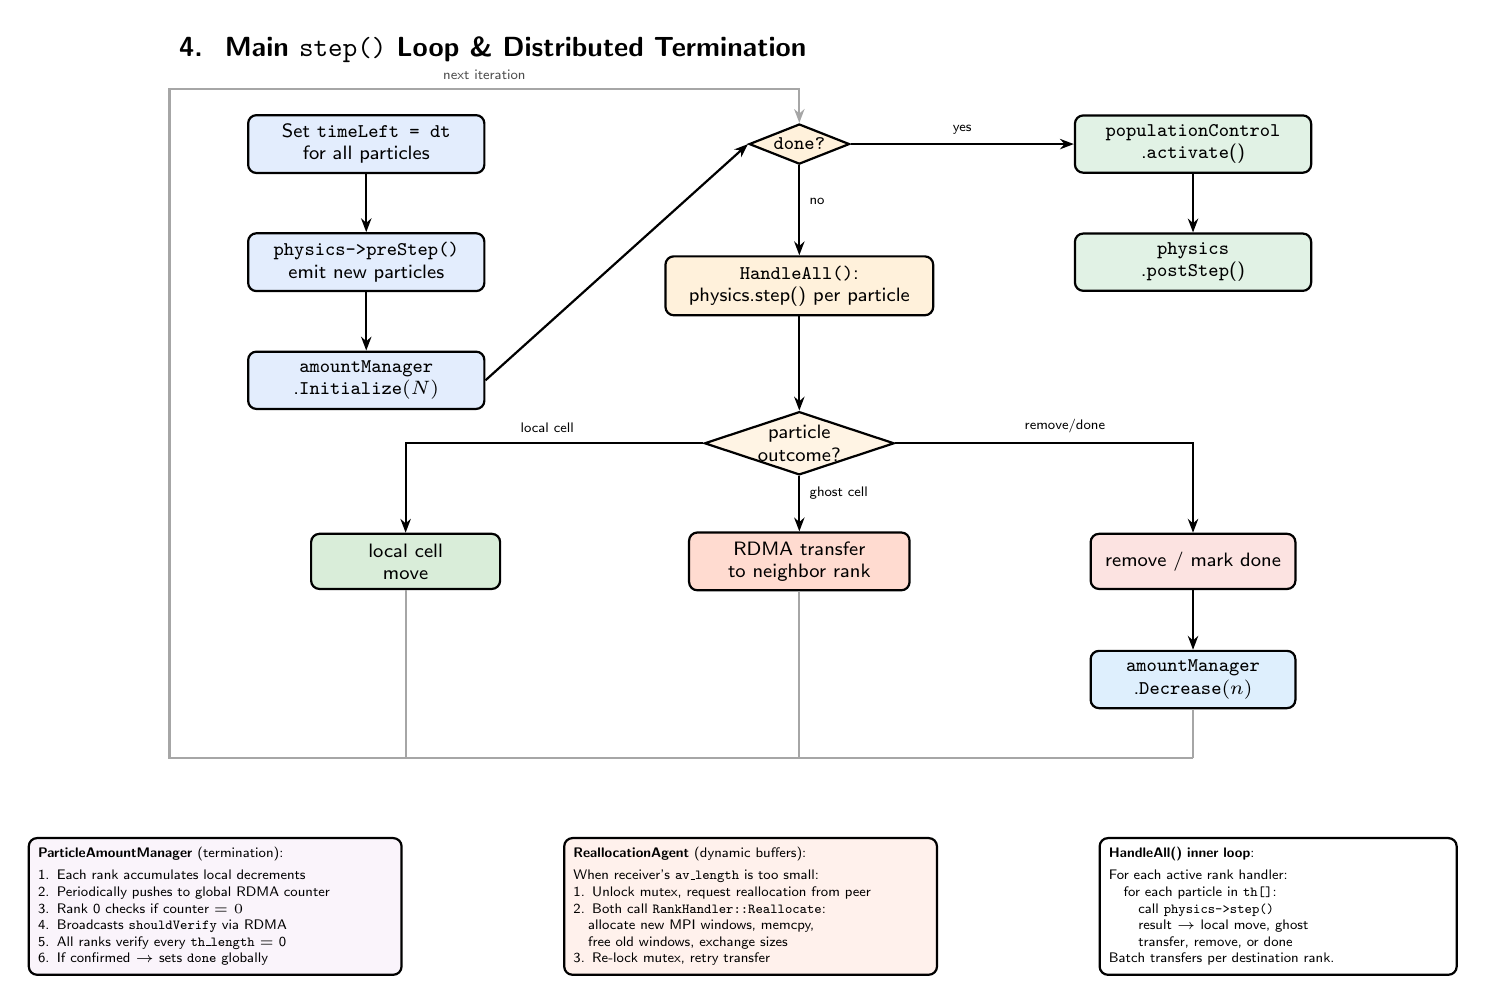
\begin{tikzpicture}[>=Stealth, font=\sffamily\small]

  \node[font=\sffamily\normalsize\bfseries, anchor=west] at (-1, 0)
    {4.\; Main \texttt{step()} Loop \& Distributed Termination};

  \begin{scope}[shift={(0, -8.5)}]
    \tikzset{
      fbox/.style={
        draw, rounded corners=3pt, thick, minimum width=3.0cm,
        minimum height=0.7cm, font=\sffamily\scriptsize, align=center
      },
      dec/.style={
        draw, diamond, thick, aspect=2.5, inner sep=1pt,
        font=\sffamily\scriptsize, align=center
      }
    }

    % ---- Left column: linear init ----
    \node[fbox, fill=rank0!15] (init) at (1.5, 7.3)
      {Set \texttt{timeLeft = dt}\\for all particles};
    \node[fbox, fill=rank0!15] (prestep) at (1.5, 5.8)
      {\texttt{physics->preStep()}\\emit new particles};
    \node[fbox, fill=rank0!15] (initcnt) at (1.5, 4.3)
      {\texttt{amountManager}\\.\texttt{Initialize}$(N)$};

    \draw[-{Stealth[length=5pt]}, thick] (init) -- (prestep);
    \draw[-{Stealth[length=5pt]}, thick] (prestep) -- (initcnt);

    % ---- Center column: main loop ----
    \node[dec, fill=thcolor!20] (done) at (7, 7.3) {\texttt{done?}};

    \draw[-{Stealth[length=5pt]}, thick] (initcnt.east) -- (done.west);

    % HandleAll
    \node[fbox, fill=thcolor!20, minimum width=3.4cm] (handle) at (7, 5.5)
      {\texttt{HandleAll()}:\\physics.step() per particle};

    \draw[-{Stealth[length=5pt]}, thick] (done.south) --
      node[right, font=\sffamily\tiny, pos=0.4] {no} (handle);

    % Outcome
    \node[dec, fill=thcolor!15, inner sep=0pt, aspect=3.0]
      (fate) at (7, 3.5) {particle\\outcome?};

    \draw[-{Stealth[length=5pt]}, thick] (handle) -- (fate);

    % ---- Three branches ----

    % Left branch: local cell move
    \node[fbox, fill=partcolor!70, minimum width=2.4cm] (local) at (2.0, 2.0)
      {local cell\\move};
    \draw[-{Stealth[length=5pt]}, thick] (fate.west) -|
      node[above left, font=\sffamily\tiny, pos=0.2] {local cell} (local.north);

    % Center branch: ghost transfer
    \node[fbox, fill=rdmacolor!25, minimum width=2.8cm] (xfer) at (7, 2.0)
      {RDMA transfer\\to neighbor rank};
    \draw[-{Stealth[length=5pt]}, thick] (fate.south) --
      node[right, font=\sffamily\tiny, pos=0.3] {ghost cell} (xfer.north);

    % Right branch: remove / done
    \node[fbox, fill=rank1!15, minimum width=2.6cm] (rem) at (12.0, 2.0)
      {remove / mark done};
    \draw[-{Stealth[length=5pt]}, thick] (fate.east) -|
      node[above right, font=\sffamily\tiny, pos=0.2] {remove/done} (rem.north);

    % Decrement below remove
    \node[fbox, fill=avcolor!30, minimum width=2.6cm] (decr) at (12.0, 0.5)
      {\texttt{amountManager}\\.\texttt{Decrease}$(n)$};
    \draw[-{Stealth[length=5pt]}, thick] (rem) -- (decr);

    % ---- Loop-back: all three rejoin at the top via a clean rectangular path ----
    \def\busY{-0.5}
    % local -> bus
    \draw[thick, gray!70] (local.south) -- (2.0, \busY);
    % xfer -> bus
    \draw[thick, gray!70] (xfer.south) -- (7, \busY);
    % decr -> bus
    \draw[thick, gray!70] (decr.south) -- (12.0, \busY);
    % horizontal bus
    \draw[thick, gray!70] (2.0, \busY) -- (12.0, \busY);
    % left side up and across the top to done.north
    \draw[-{Stealth[length=5pt]}, thick, gray!70]
      (2.0, \busY) -- (-1.0, \busY) -- (-1.0, 8.0) -- (7, 8.0) -- (done.north);
    \node[font=\sffamily\tiny, gray!60!black, anchor=south] at (3, 8.0)
      {next iteration};

    % ---- Exit: done = yes ----
    \node[fbox, fill=rank2!15] (popctl) at (12.0, 7.3)
      {\texttt{populationControl}\\.\texttt{activate}()};
    \node[fbox, fill=rank2!15] (post) at (12.0, 5.8)
      {\texttt{physics}\\.\texttt{postStep}()};

    \draw[-{Stealth[length=5pt]}, thick] (done.east) --
      node[above, font=\sffamily\tiny] {yes} (popctl.west);
    \draw[-{Stealth[length=5pt]}, thick] (popctl) -- (post);

    % ---- Side boxes: termination & reallocation ----
    \node[draw, rounded corners=3pt, fill=mutexcolor!10, thick,
          font=\sffamily\tiny, text width=4.5cm, align=left,
          anchor=north west] at (-2.8, -1.5) {
      \textbf{ParticleAmountManager} (termination):\\[2pt]
      1. Each rank accumulates local decrements\\
      2. Periodically pushes to global RDMA counter\\
      3. Rank 0 checks if counter $= 0$\\
      4. Broadcasts \texttt{shouldVerify} via RDMA\\
      5. All ranks verify every \texttt{th\_length}~$=$~0\\
      6. If confirmed $\to$ sets \texttt{done} globally
    };

    \node[draw, rounded corners=3pt, fill=rdmacolor!10, thick,
          font=\sffamily\tiny, text width=4.5cm, align=left,
          anchor=north west] at (4.0, -1.5) {
      \textbf{ReallocationAgent} (dynamic buffers):\\[2pt]
      When receiver's \texttt{av\_length} is too small:\\
      1. Unlock mutex, request reallocation from peer\\
      2. Both call \texttt{RankHandler::Reallocate}:\\
      \quad allocate new MPI windows, memcpy,\\
      \quad free old windows, exchange sizes\\
      3. Re-lock mutex, retry transfer
    };

    \node[draw, rounded corners=3pt, fill=white, thick,
          font=\sffamily\tiny, text width=4.3cm, align=left,
          anchor=north west] at (10.8, -1.5) {
      \textbf{HandleAll() inner loop}:\\[2pt]
      For each active rank handler:\\
      \quad for each particle in \texttt{th[]}:\\
      \quad\quad call \texttt{physics->step()}\\
      \quad\quad result $\to$ local move, ghost\\
      \quad\quad transfer, remove, or done\\
      Batch transfers per destination rank.
    };
  \end{scope}

\end{tikzpicture}

\end{document}
